\documentclass[12]{article} %the sets the document type.

\usepackage{amsmath,amssymb,amsthm} %this loads commonly used math packages
\usepackage{enumitem}
\usepackage{float}
\newtheorem{theorem}{Theorem} %this declares the theorem environment
\setlist[enumerate]{leftmargin=*,widest=0}
\usepackage{graphicx}
\graphicspath{ {boolesResources/} }

\title{George Boole}
\author{Nick Zayatz and Michele Burns}

\renewcommand{\baselinestretch}{1.5} 
\begin{document} %document starts here
\maketitle % makes the title

Over the course of his life, George Boole made some major contributions to mathematics. In the field of analysis, Boole published his treatise \textit{Applications to the Theory of Definite Integrals On the Comparison of Transcendents, with Certain Applications to the Theory of Definite Integrals} in 1857. In this work, Boole mainly studies the sum of residues of rational functions. A residue is most simply described as a complex number that is proportional to the line integral of a complex function that is complexly differentiable on its entire domain except for a few select points. These residues are calculated by functions in the form $f: \mathbb{C}\setminus \{a_{k}\}_{k} \rightarrow \mathbb{C}$, where $f$ is complexly differentiable on all points except $\{a_{k}\}_{k}$. Boole's work in this field eventually lead him to the equality which we not call Boole's Identity. This identity states that $\forall a_{k},b_{k}, \text{ and } t \in \mathbb{R}$ where $a_{k} > 0 \text{ and } t > 0$, then the following identity is true:

\begin{figure}[H]
\centerline{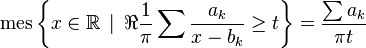
\includegraphics[scale=0.8]{boolesIdentity}.}
\caption{Boole's Identity for residues of rational functions.}\label{fig1}
\end{figure}

Boole also did some minor work in the study of probability. In the second part of his "An Investigation of The Laws of Thought" (1854), Boole used his new discoveries in symbolic logic in an attempt to determine whether or not events would happen based on what passed events had previously occurred. This section of his work contains the proof of the \textbf{union bound}, otherwise know as Boole's Inequality.

Despite his contributions to other mathematical fields, Boole most important addition to the field of mathematics was his work involving symbolic logic, which many now refer to as "Boolean Algebra." Boole first introduced this topic of study in his treatise "The Mathematical Analysis of Logic" in 1847. The idea was then further expanded and refined in 1854, when Boole published his most famous work "An Investigation of The Laws of Thought."

\newpage



\begin{thebibliography}{9}
\bibitem{AnalysisBook} 
Boole, George. 
\textit{Applications to the Theory of Definite Integrals On the Comparison of Transcendents, with Certain Applications to the Theory of Definite Integrals}. 
London: Philosophical Transactions, 1857. 745-803. Print.
 
\bibitem{BooleanBook2} 
Boole, George. 
\textit{An Investigation of the Laws of Thought: On Which Are Founded Mathematical Theories of Logic and Probabilities}.
New York: Dover, 1854. Print.
 
\bibitem{MacTutor} 
"George Boole."
\textit{Boole Biography}.
JOC/EFR, June 2004. Web. 16 Feb. 2016. 
\end{thebibliography}

\end{document}